\section{Test af GPU-calculate}
Der er lavet 2 test inden for \textit{Funcalc} der har en stor lighed med hinanden. den første test er kolonne \textit{A} fyldt med konstanter, tallet 2, og kolonne \textit{B} fyldt med konstanter, tallet 3. I kolonne \textit{C} er der hvor udregningen vil ske. Denne test starter med \textit{A1*B1} og for ver \textit{x} bliver der liget et ekstra \textit{+A1*B1} på udregningen.

I Test to er kolonnerne \textit{A} og \textit{B} fyldt med tallet 2 og kolonnerne \textit{C} og \textit{D} fyldt med tallet 3. Kolonne \textit{E} bliver brugt til at holde udregningerne i, hvor denne test starter med Denne test starter med \textit{A1*B1*C1*D1} og for ver \textit{x} bliver der liget et ekstra \textit{+A1*B1*C1*D1} på udregningen.

\subsection{Resultater}
på tabel \ref{fig:Funcalc_test_2} kan resultaterne fra første test ses og på tabel \ref{fig:Funcalc_test_1} kan resultaterne fra første test ses


% ------------------------------------------------------------------------------------------------------------- Funcalc test 2
\begin{figure}[p]
    \centering
   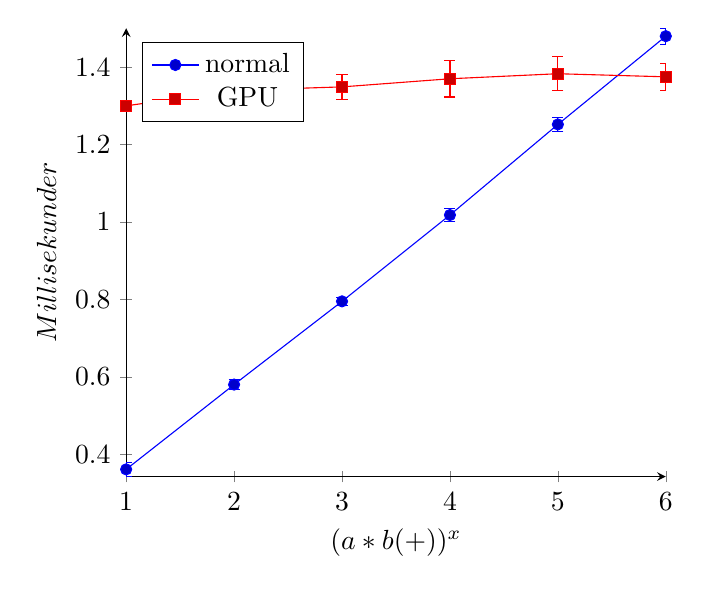
\begin{tikzpicture} 
\begin{axis}
[
    axis lines = left,
    xlabel = $ (a*b(+))^x $,
    ylabel = $Millisekunder$,
    legend pos=north west,
]

\addplot+[error bars/.cd,y dir=both,y explicit]
	coordinates 
    	{ 	
		(1,0.36100000000000004) +- (0,0.018529256146248507)
		(2,0.58000000000000007) +- (0,0.01247219128923985)
		(3,0.795) +- (0, 0.010801234497347552)
		(4,1.018) +- (0,0.016865480854228086)
		(5,1.2520000000000002) +- (0,0.018135294011630478)
		(6,1.48) +- (0,0.020548046676568125)
 }; \addlegendentry{normal}
 
 \addplot+[error bars/.cd,y dir=both,y explicit]
	coordinates 
    	{ 	
		(1,1.3) +- (0,0.01154700538377906)
		(2,1.3400000000000003) +- (0,0.039999999999992868)
		(3,1.349) +- (0, 0.032812599206197689)
		(4,1.3699999999999999) +- (0,0.047140452079106852)
		(5,1.3829999999999998) +- (0,0.043982319680124123)
		(6,1.375) +- (0,0.035355339059328042)
 }; \addlegendentry{GPU}
\end{axis} \end{tikzpicture}    
    \caption{testen af Funcalc hvor kolonerne er fyldt ud, 1000 tal i vær kolonne, hvor \textit{A=2},\textit{B=3} og C er hvor funktioner ligger. \textit{x} står for hvor mange udredninger der er af  (a1*b1(+)) og for GPU (1*2(+)) .}
    \label{fig:Funcalc_test_2}
\end{figure}

% ------------------------------------------------------------------------------------------------------------- Funcalc test 1
\begin{figure}[p]
    \centering
   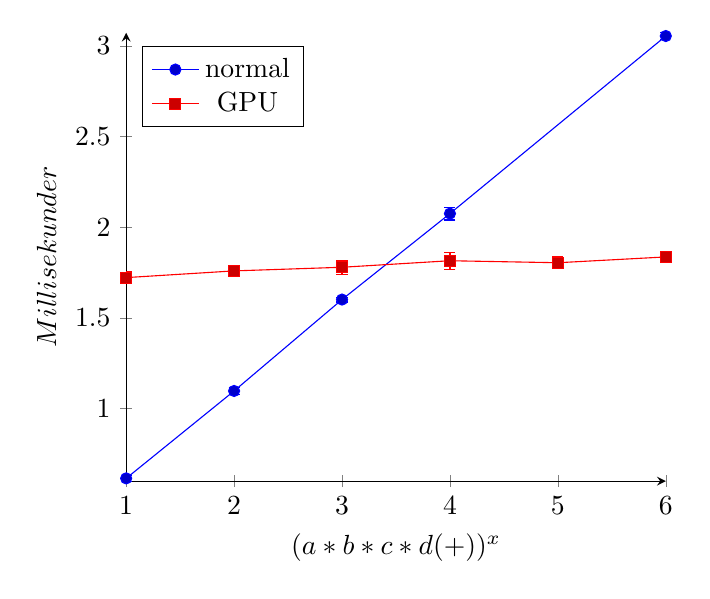
\begin{tikzpicture} 
\begin{axis}
[
    axis lines = left,
    xlabel = $ (a*b*c*d(+))^x $,
    ylabel = $Millisekunder$,
    legend pos=north west,
]

\addplot+[error bars/.cd,y dir=both,y explicit]
	coordinates 
    	{ 	
		(1,0.615) +- (0,0.015092308563562756)
		(2,1.097) +- (0,0.017669811040937646)
		(3,1.6010000000000002) +- (0, 0.013703203194048448)
		(4,2.075) +- (0.019578900207433445)
		(5,2.572) +- (0,0.035527766918592094)
		(6,3.0539999999999994) +- (0,0.017763883459407156)
 }; \addlegendentry{normal}
 \addplot+[error bars/.cd,y dir=both,y explicit]
	coordinates 
    	{ 	
		(1,1.722) +- (0,0.031198290551458049)
		(2,1.759) +- (0,0.026853512081510652)
		(3,1.779) +- (0,0.038137179293238864)
		(4,1.815) +- (0,0.0460072458061408788)
		(5,1.8040000000000003) +- (0,0.03306559138036088)
		(6,1.8359999999999999) +- (0,0.030258148581095181)
 }; \addlegendentry{GPU}
\end{axis} \end{tikzpicture}    
    \caption{testen af Funcalc hvor kolonerne er fyldt ud, 1000 tal i vær kolonne, hvor \textit{A=B=2},\textit{C=D=3} og E er hvor funktioner ligger. \textit{x} står for hvor mange udredninger der er af  (a1*b1*c1*d1(+)) og for GPU (1*2*3*4(+)).}
    \label{fig:Funcalc_test_1}
\end{figure}

